% =====================================================================
\section{Kết quả phần mở rộng: Contrastive Learning và SupCon}
\label{sec:results-ext}
% =====================================================================

Phần này trình bày khối mở rộng tùy chọn \cfg{E3}--\cfg{E6} đã mô tả tại
\secref{sec:contrastive}, chạy \emph{sau} khi khối đối chứng chính đã hoàn tất. Đây là phần
nằm ngoài yêu cầu bắt buộc của đề cương, nên mọi kết luận ở đây được trình bày như
\textbf{bằng chứng thăm dò} chứ không phải kết luận của đề tài.

\subsection{Nguyên tắc khóa siêu tham số}
\label{sec:results-ext-lambda}

Điều khoản 4.2 của đề cương yêu cầu khóa siêu tham số mở rộng bằng validation trước khi đánh
giá test, và cấm lựa chọn cấu hình dựa trên kết quả test. Vì vậy quy trình được chia thành hai
bước tách bạch về mặt thông tin:

\begin{enumerate}[label=\textbf{B\arabic*.},leftmargin=1.4cm,itemsep=3pt]
  \item \textbf{Khảo sát chỉ trên validation.} Chạy \cfg{E4} và \cfg{E6} tại mức
        $10\,\%$ nhãn, seed 42, với $\lamc \in \{0{,}05;\ 0{,}1;\ 0{,}25;\ 0{,}5;\ 1{,}0\}$.
        Script khảo sát (\code{scripts/sweep\_lambda\_c.py}) \textbf{không gọi} bước đánh giá
        test, nên kết quả test không thể ảnh hưởng tới quyết định.
  \item \textbf{Khóa $\lamc$} theo một quy tắc khai báo trước: chọn \emph{một} giá trị dùng
        chung cho mọi cấu hình mở rộng (đúng như bảng 5 của đề cương) sao cho \emph{trung bình}
        Macro-F1 validation qua hai cấu hình khảo sát là lớn nhất. Quy tắc này được chọn vì mỗi
        cấu hình có cực trị riêng (xem \tabref{tab:lambda-sweep}); khóa theo một cấu hình duy
        nhất có thể rất kém cho cấu hình còn lại.
\end{enumerate}

% Sinh tự động — scripts/make_report_data.py
\begin{table}[htbp]
  \centering
  \small
  \begin{tabular}{@{}l c c c c c@{}}
    \toprule
    Cấu hình & $\lambda_c = 0,05$ & $\lambda_c = 0,10$ & $\lambda_c = 0,25$ & $\lambda_c = 0,50$ & $\lambda_c = 1,00$ \\
    \midrule
    \cfg{E4} & 0,9266 & 0,9354 & 0,9352 & 0,9425 & 0,9454 \\
    \cfg{E6} & 0,9391 & 0,9418 & 0,9496 & 0,9457 & 0,9468 \\
    \midrule
    \textit{được khóa} &  &  &  &  & $\bullet$ \\
    \bottomrule
  \end{tabular}
  \caption{Khảo sát $\lambda_c$ bằng \textbf{Macro-F1 validation} với 40 epoch, mức 10\,\% nhãn, seed 42. Tập test \textbf{không} được đánh giá trong bước này. Quy tắc khóa được khai báo trước: chọn \emph{một} $\lambda_c$ dùng chung cho mọi cấu hình mở rộng sao cho trung bình Macro-F1 validation qua hai cấu hình khảo sát là lớn nhất; giá trị được chọn là 1,00 (trung bình 0,9461).}
  \label{tab:lambda-sweep}
\end{table}

\figref{fig:lambda-sweep} cho thấy toàn bộ đường khảo sát. Đáng lưu ý, cả hai hàm mất mát đều
\emph{nhạy} với $\lamc$: chênh lệch giữa giá trị tốt nhất và xấu nhất trong lưới khảo sát là
khoảng $2$ điểm phần trăm Macro-F1 validation. Điều này khẳng định việc chạy khảo sát là cần
thiết, thay vì chọn $\lamc$ theo trực giác.

\begin{figure}[htbp]
  \centering
  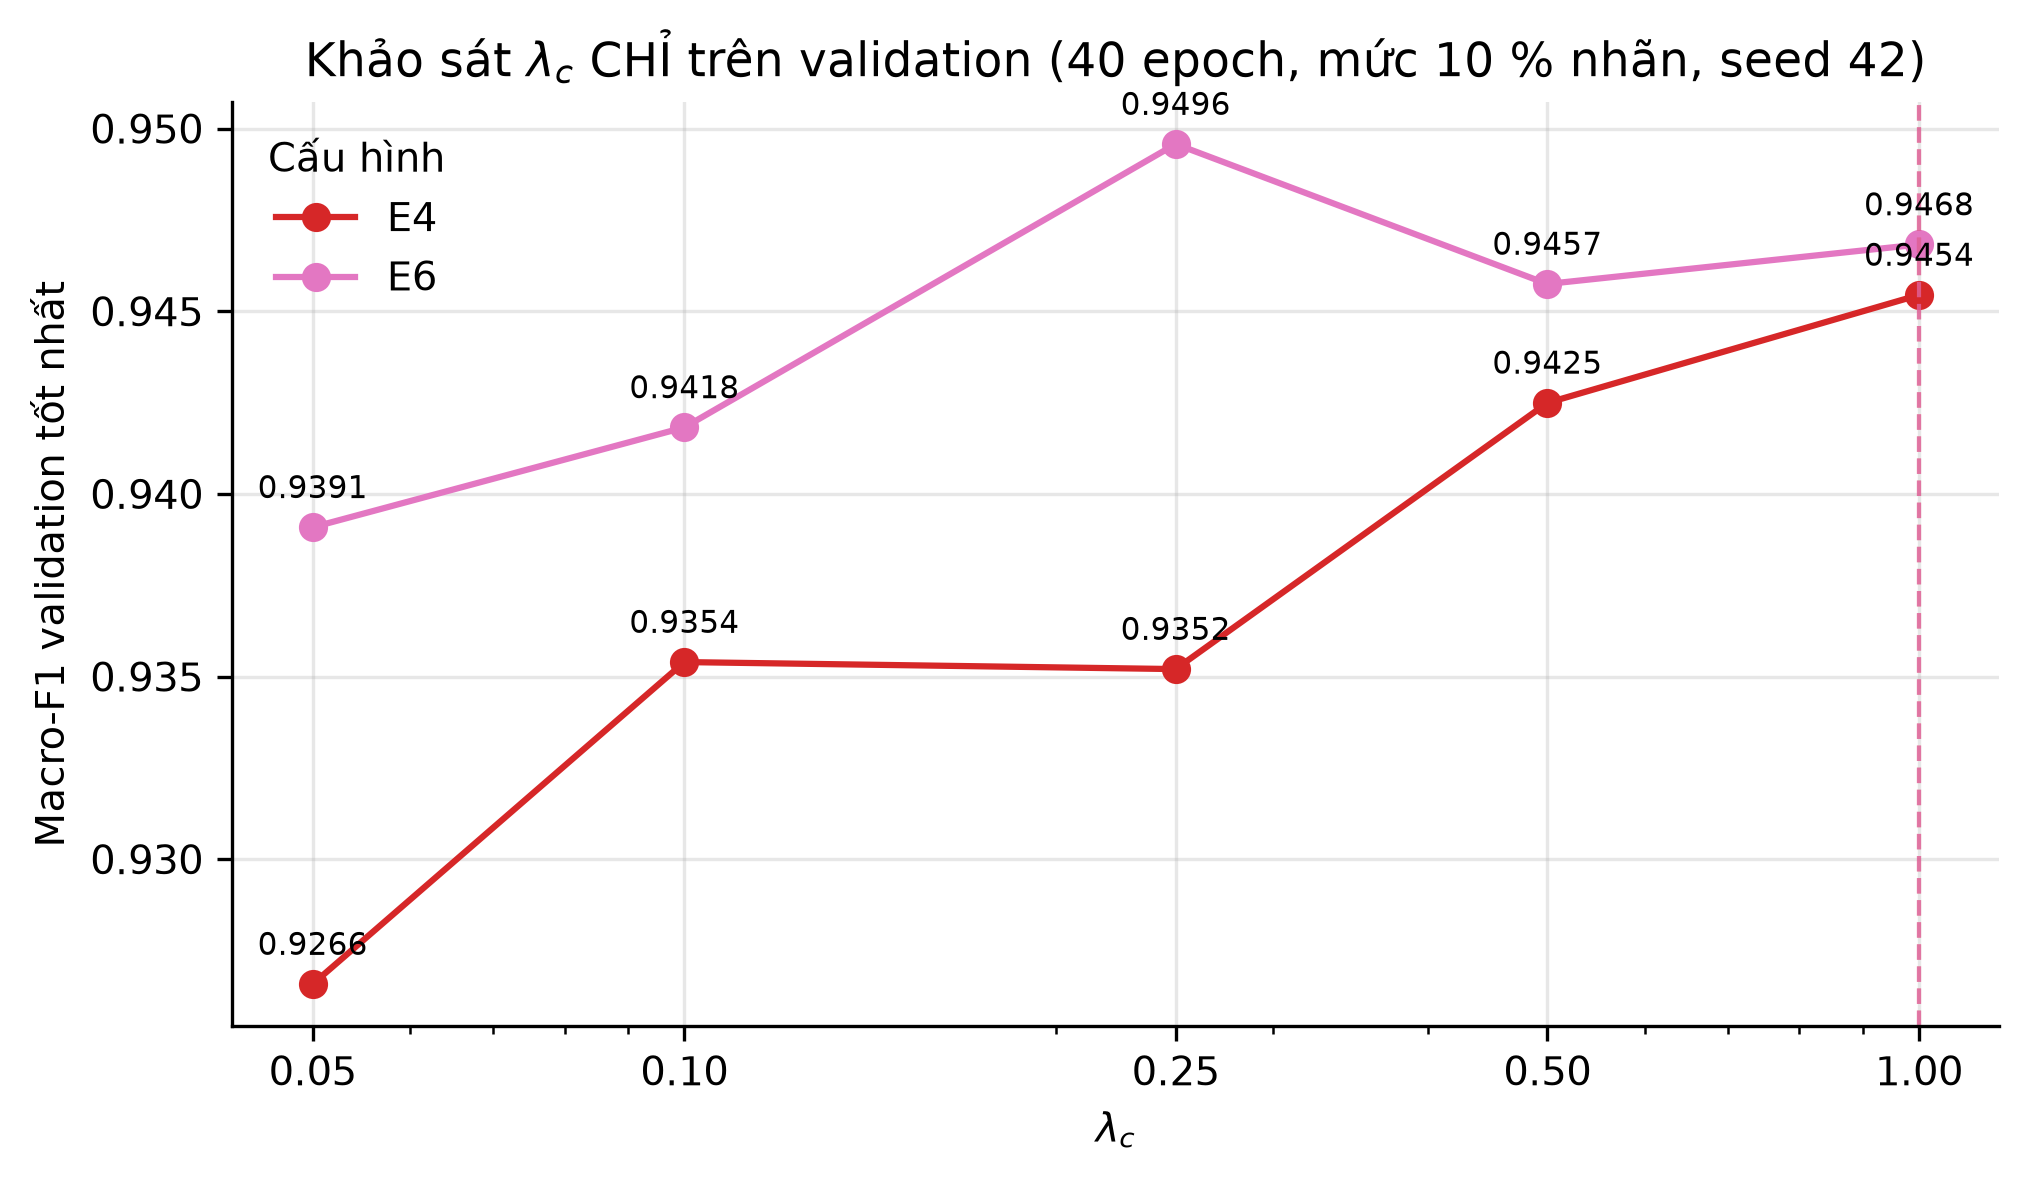
\includegraphics[width=0.92\textwidth]{../results/figures/fig08_lambda_sweep.png}
  \caption{Khảo sát $\lamc$ \textbf{chỉ trên Macro-F1 validation} (40 epoch, mức
  $10\,\%$ nhãn, seed 42). Đường đứt dọc là giá trị được khóa. Tập test không được đánh giá
  trong bước này.}
  \label{fig:lambda-sweep}
\end{figure}

\subsection{Kết quả và đối chứng ghép cặp}
\label{sec:results-ext-main}

Sau khi khóa $\lamc$, bốn cấu hình được chạy tại mức nhãn \textbf{$10\,\%$} với ba lần lặp
42, 43, 44 — tổng cộng $4 \times 3 = 12$ lượt huấn luyện 100 epoch. Mức $10\,\%$ được chọn vì
đây là mức ưu tiên của đề cương (mục 4.2) và là mức mà phần bắt buộc cho thấy độ biến động lớn
nhất giữa các cấu hình. Mỗi lượt vẫn giữ đúng giao thức của khối chính: 100 epoch, AdamW, chọn
checkpoint bằng Macro-F1 validation, không Early Stopping, không dùng test-time augmentation.

\begin{keybox}
\textbf{Giới hạn phạm vi.} Khối mở rộng chỉ được chạy ở mức $10\,\%$ nhãn; hai mức $20\,\%$ và
$50\,\%$ \textbf{không} được khảo sát cho \cfg{E3}--\cfg{E6}. Vì vậy mọi kết luận ở
\secref{sec:results-ext} \emph{chỉ} áp dụng cho mức $10\,\%$ nhãn, kiến trúc và giao thức đã mô
tả. So sánh với \cfg{E1} vẫn hợp lệ vì \cfg{E1} có kết quả đầy đủ ở cả ba mức nhãn.
\end{keybox}

% Sinh tự động — scripts/make_report_data.py
\begin{table}[htbp]
  \centering
  \scriptsize
  \setlength{\tabcolsep}{4.5pt}
  \begin{tabular}{@{}l r r r r r r@{}}
    \toprule
    & \multicolumn{2}{c}{10\,\% nhãn} & \multicolumn{2}{c}{20\,\% nhãn} & \multicolumn{2}{c}{50\,\% nhãn} \\
    \cmidrule(lr){2-3}\cmidrule(lr){4-5}\cmidrule(lr){6-7}
    Cấu hình & Macro-F1 & $\Delta$ & Macro-F1 & $\Delta$ & Macro-F1 & $\Delta$ \\
    \midrule
    \cfg{E1} & 0,9319 & --- & 0,9497 & --- & 0,9690 & --- \\
    \addlinespace[2pt]
    \cfg{E2-L} & 0,9313 & $-$0,06 & 0,9505 & +0,08 & 0,9745 & +0,55 \\
    \addlinespace[2pt]
    \cfg{E2} & 0,9470 & +1,51 & 0,9631 & +1,34 & 0,9777 & +0,88 \\
    \cfg{E3} & 0,9438 & +1,19 & --- & --- & --- & --- \\
    \cfg{E4} & 0,9527 & +2,07 & --- & --- & --- & --- \\
    \cfg{E5} & 0,9496 & +1,77 & --- & --- & --- & --- \\
    \cfg{E6} & 0,9579 & +2,60 & --- & --- & --- & --- \\
    \bottomrule
  \end{tabular}
  \caption{Kết quả trên $\Dtest$, trung bình qua ba lần lặp. $\Delta$ là chênh lệch Macro-F1 ghép cặp so với \cfg{E1} ở cùng mức nhãn, đơn vị điểm phần trăm. Hai nhóm được ngăn bằng khoảng trắng: \cfg{E1}/\cfg{E2-L}/\cfg{E2} là khối chính; \cfg{E3}--\cfg{E6} là khối mở rộng contrastive.}
  \label{tab:extension-results}
\end{table}

\begin{figure}[htbp]
  \centering
  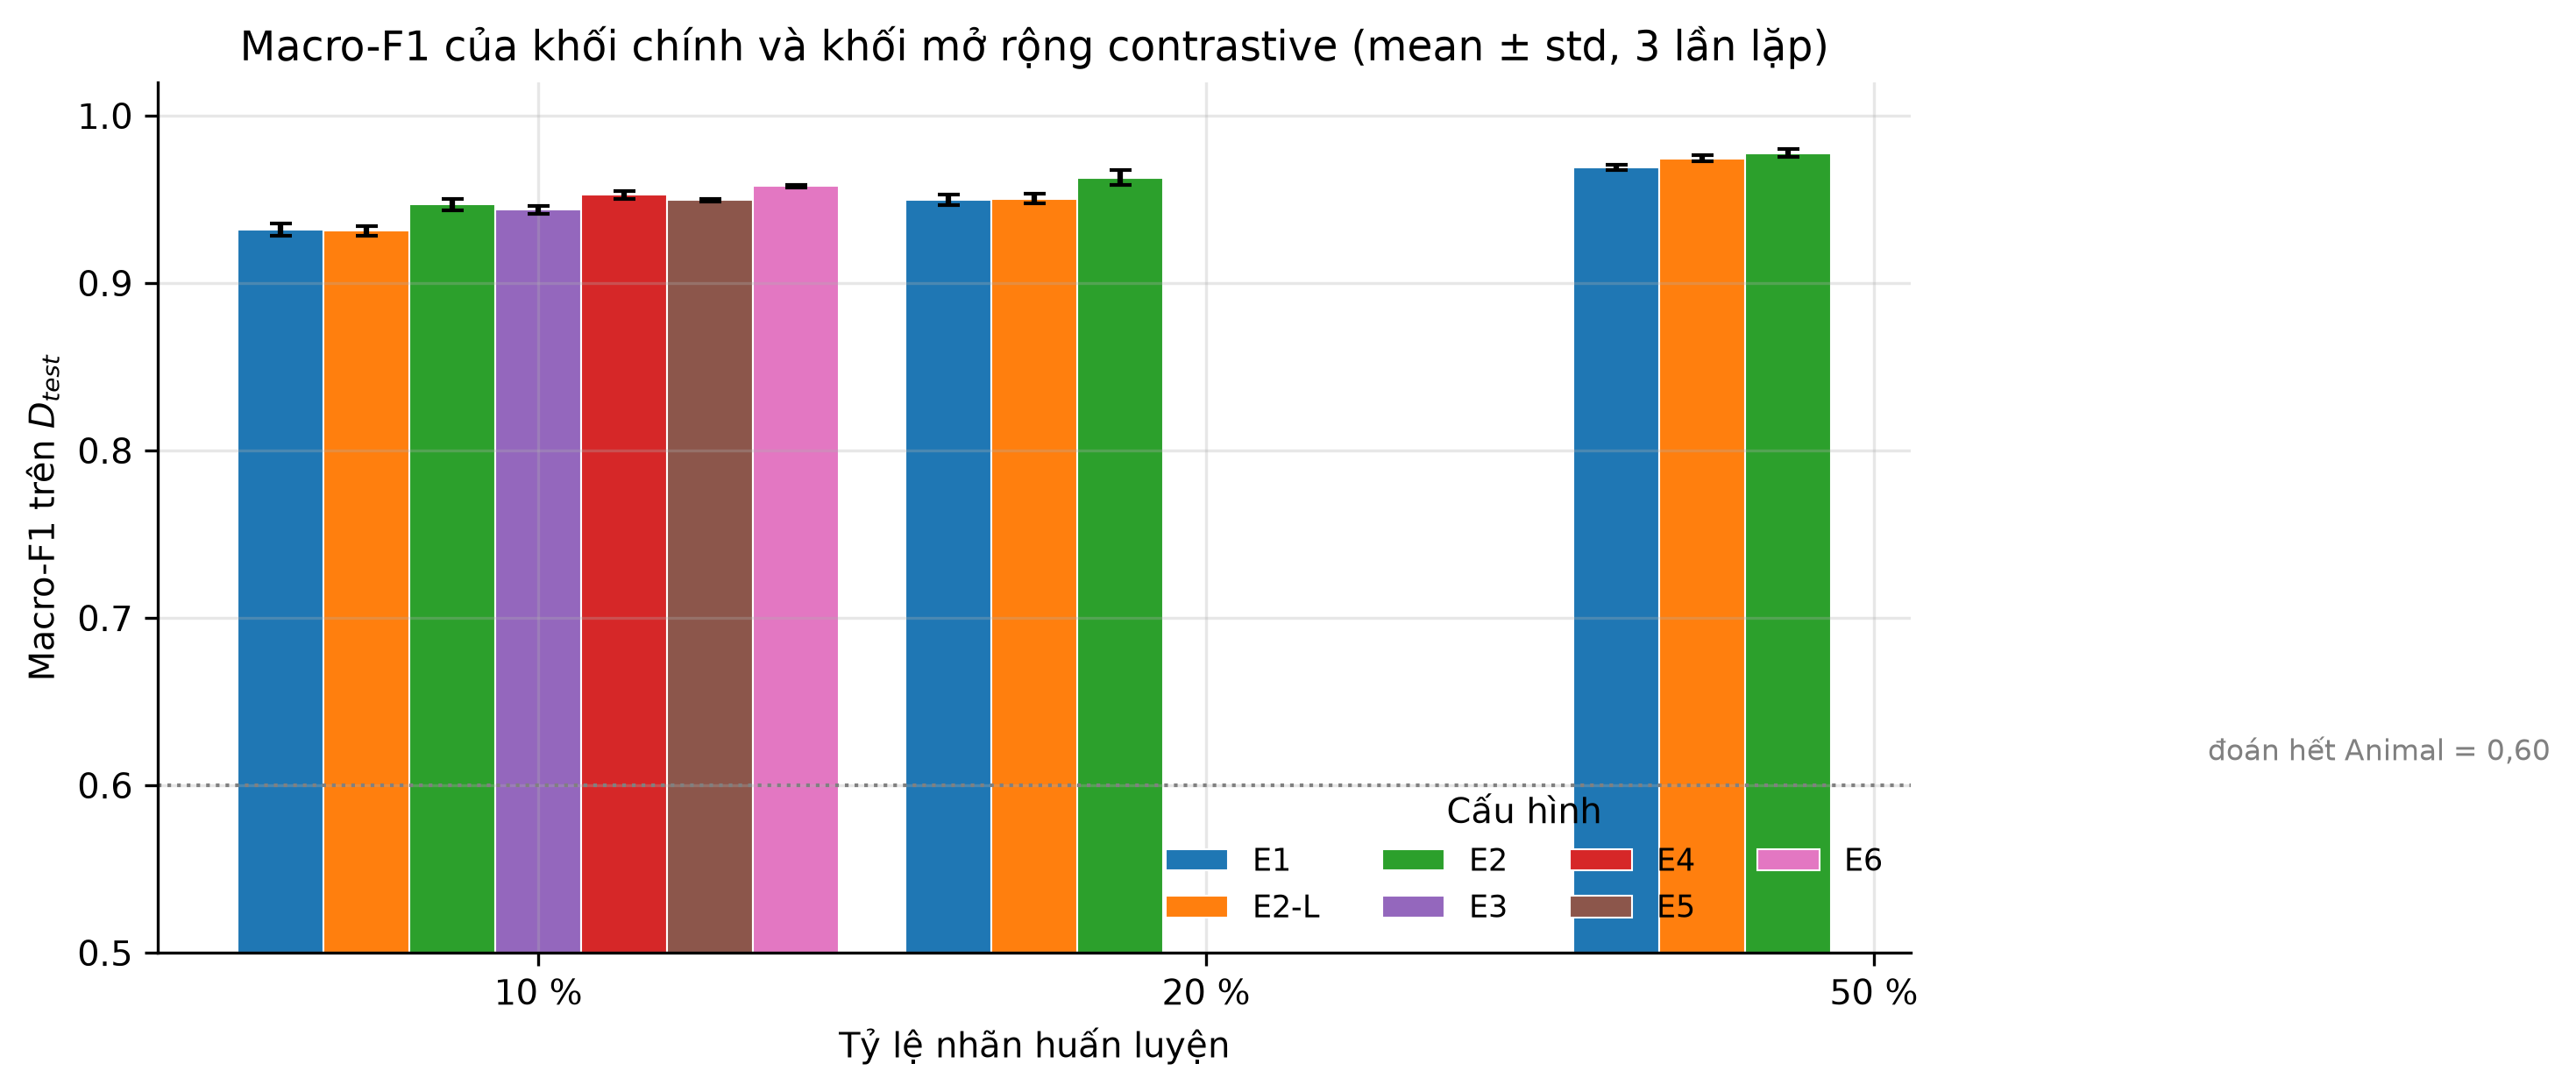
\includegraphics[width=\textwidth]{../results/figures/fig06_extension_macro_f1.png}
  \caption{Macro-F1 trên $\Dtest$ của các cấu hình \emph{đã có kết quả}, trung bình qua các lần
  lặp đã xong, so với mức $0{,}60$ của bộ phân loại luôn đoán Animal. Khối chính (\cfg{E1},
  \cfg{E2-L}, \cfg{E2}) có kết quả ở cả ba mức nhãn; khối mở rộng contrastive chỉ được khảo sát
  ở mức $10\,\%$ nhãn (xem \tabref{tab:extension-results}). Hình được sinh lại tự động bởi
  \code{scripts/make\_extension\_figures.py}, nên số cột phản ánh đúng số cấu hình đã chạy
  xong tại thời điểm sinh báo cáo.}
  \label{fig:extension-f1}
\end{figure}

\begin{figure}[htbp]
  \centering
  
\includegraphics[width=\textwidth]{../results/figures/fig07_extension_delta.png}
  \caption{Chênh lệch ghép cặp $\Delta_s$ so với \cfg{E1} của từng cấu hình mở rộng, mỗi điểm
  là một lần lặp. Đường ngang là trung bình các lần lặp đã xong. Giá trị dương nghĩa là cấu hình
  đó tốt hơn baseline ở cùng ngân sách nhãn. Nếu chưa có lượt mở rộng nào thì hình chỉ hiển thị
  thông báo chưa có dữ liệu — đây là hình sinh tự động, không phải hình minh hoạ.}
  \label{fig:extension-delta}
\end{figure}

\subsection{Phân tích}
\label{sec:results-ext-analysis}

\RExtensionAnalysis

\subsection{Chi phí của phần mở rộng}
\label{sec:results-ext-cost}

% Sinh tự động — scripts/make_report_data.py
\begin{table}[htbp]
  \centering
  \scriptsize
  \setlength{\tabcolsep}{4pt}
  \begin{tabular}{@{}l r r r r r@{}}
    \toprule
    Cấu hình & \makecell[r]{Tham số\\suy luận} & \makecell[r]{Rotation\\Head} & \makecell[r]{Projection\\Head} & \makecell[r]{Giây/epoch\\(mức 10\,\%)} & \makecell[r]{Lượt ảnh phụ\\mỗi epoch\\(mức 10\,\%)} \\
    \midrule
    \cfg{E1} & 11.169.858 & 0 & 0 & 3,4 & 0 \\
    \cfg{E2-L} & 11.169.858 & 2.052 & 0 & 5,8 & 4.608 \\
    \cfg{E2} & 11.169.858 & 2.052 & 0 & 5,8 & 4.608 \\
    \cfg{E3} & 11.169.858 & 0 & 328.832 & 15,0 & 9.000 \\
    \cfg{E4} & 11.169.858 & 0 & 328.832 & 15,1 & 9.000 \\
    \cfg{E5} & 11.169.858 & 2.052 & 328.832 & 17,9 & 13.500 \\
    \cfg{E6} & 11.169.858 & 2.052 & 328.832 & 18,2 & 13.500 \\
    \bottomrule
  \end{tabular}
  \caption{Chi phí của khối mở rộng. Số tham số suy luận \textbf{không} thay đổi so với khối chính vì cả Rotation Head lẫn Projection Head đều bị bỏ khi suy luận. \enquote{Lượt ảnh phụ} là tổng số lượt ảnh mà các nhánh phụ xử lý trong một epoch; đây là lý do định lượng khiến các cấu hình mở rộng chậm hơn \cfg{E1}.}
  \label{tab:extension-cost}
\end{table}

\paragraph{Projection Head không làm mô hình suy luận lớn hơn.}
Bảng \ref{tab:extension-cost} cho thấy số tham số suy luận của mọi cấu hình \cfg{E3}--\cfg{E6}
vẫn đúng bằng \RParamInference{} như khối chính. Cả Rotation Head lẫn Projection Head đều
\textbf{bị bỏ hoàn toàn} khi suy luận, nên chi phí thêm chỉ là chi phí học một lần. Đây là
điểm khác biệt căn bản so với các kỹ thuật tăng kích thước mô hình để tăng độ chính xác.

\paragraph{Nhánh phụ đắt hơn trong giai đoạn học.}
Các nhánh phụ khiến mỗi bước cập nhật phải xử lý thêm ảnh: nhánh xoay xử lý một minibatch,
nhánh contrastive xử lý \emph{hai} view cho mỗi ảnh trong minibatch của nó. Vì mỗi epoch vẫn
chỉ duyệt $\DL$ một lần, thời gian mỗi epoch tăng gần như tuyến tính theo số lượt ảnh phụ.

\subsection{Kết luận của phần mở rộng}
\label{sec:results-ext-conclusion}

\RExtensionConclusion
